\documentclass{mpaper}

\newtheorem{definition}{Definition}[section]
\newtheorem{corollary}{Corollary}[section]
\newtheorem{theorem}{Theorem}[section]
\newtheorem{lemma}{Lemma}[section]

\begin{document}

\title{Counting Monochromatic Components in Adversarial Graph Burning}
\author{Lewis Dyer}
\matricnum{2299195}

\maketitle

\begin{abstract}
%very rough for now
We introduce adversarial graph burning, an extension of the graph burning process to contagion with competition. We develop multiple results on the number of monochromatic components on graph colourings resulting from adversarial graph burning.

%According to Simon Peyton Jones, an abstract should address
%four key questions. First, what is the problem that this
%paper tackles? Second, why is this an interesting problem?
%Third, what is the solution this paper proposes?
%Finally, why is the proposed solution a good one?
\end{abstract}

\section{Introduction}

This paper outlines the standard template for an MSci submission.
In earlier years, MSci students at the School of Computing
Science\footnote{\url{http://www.dcs.gla.ac.uk}},
University of Glasgow, were expected to produce a full-length
dissertation. Now, the requirement is for MSci students to
write a paper of up to 14 pages in length, using the supplied
\texttt{mpaper} \LaTeX style file.

The precise structure of an MSci paper is not mandated, but it should
probably cover in detail the following aspects of the project.
\begin{enumerate}
\item General description of the problem, motivation, relevance
\item Background information, possibly including a literature survey
\item Description of approach taken to solve the problem, including
  high-level design and lower-level implementation details as appropriate
\item Evaluation, qualitative or quantitative as appropriate
\item Conclusion, including scope for future work
\end{enumerate}

\section{Background}

This \LaTeX template is based on the ACM \texttt{sig-alternate} class.
The layout is two-column text. Generally figures and tables only
extend to one column width, e.g.\ Table \ref{tab-eg},
but it is possible to make them
stretch over both columns using the \texttt{figure*} and
\texttt{table*} environments. For an example, see Figure \ref{fig-eg}.

\begin{table}
\begin{tabular}{l||c||p{2cm}}
\emph{Operating System} & \emph{Version} & \emph{Verdict} \\ \hline \hline
Ubuntu & 12.04 & Everyone's favourite Linux, unless you grew up with
RedHat \\ \hline
Slackware & xxx & Pseudo-hacker's Linux, how often do you recompile
your kernel? \\ \hline
Mac OS & 10.7 & For people with more money than sense \\ \hline
\end{tabular}
\caption{\label{tab-eg}Single column table of figures}
\end{table}

\begin{figure*}
\begin{center}
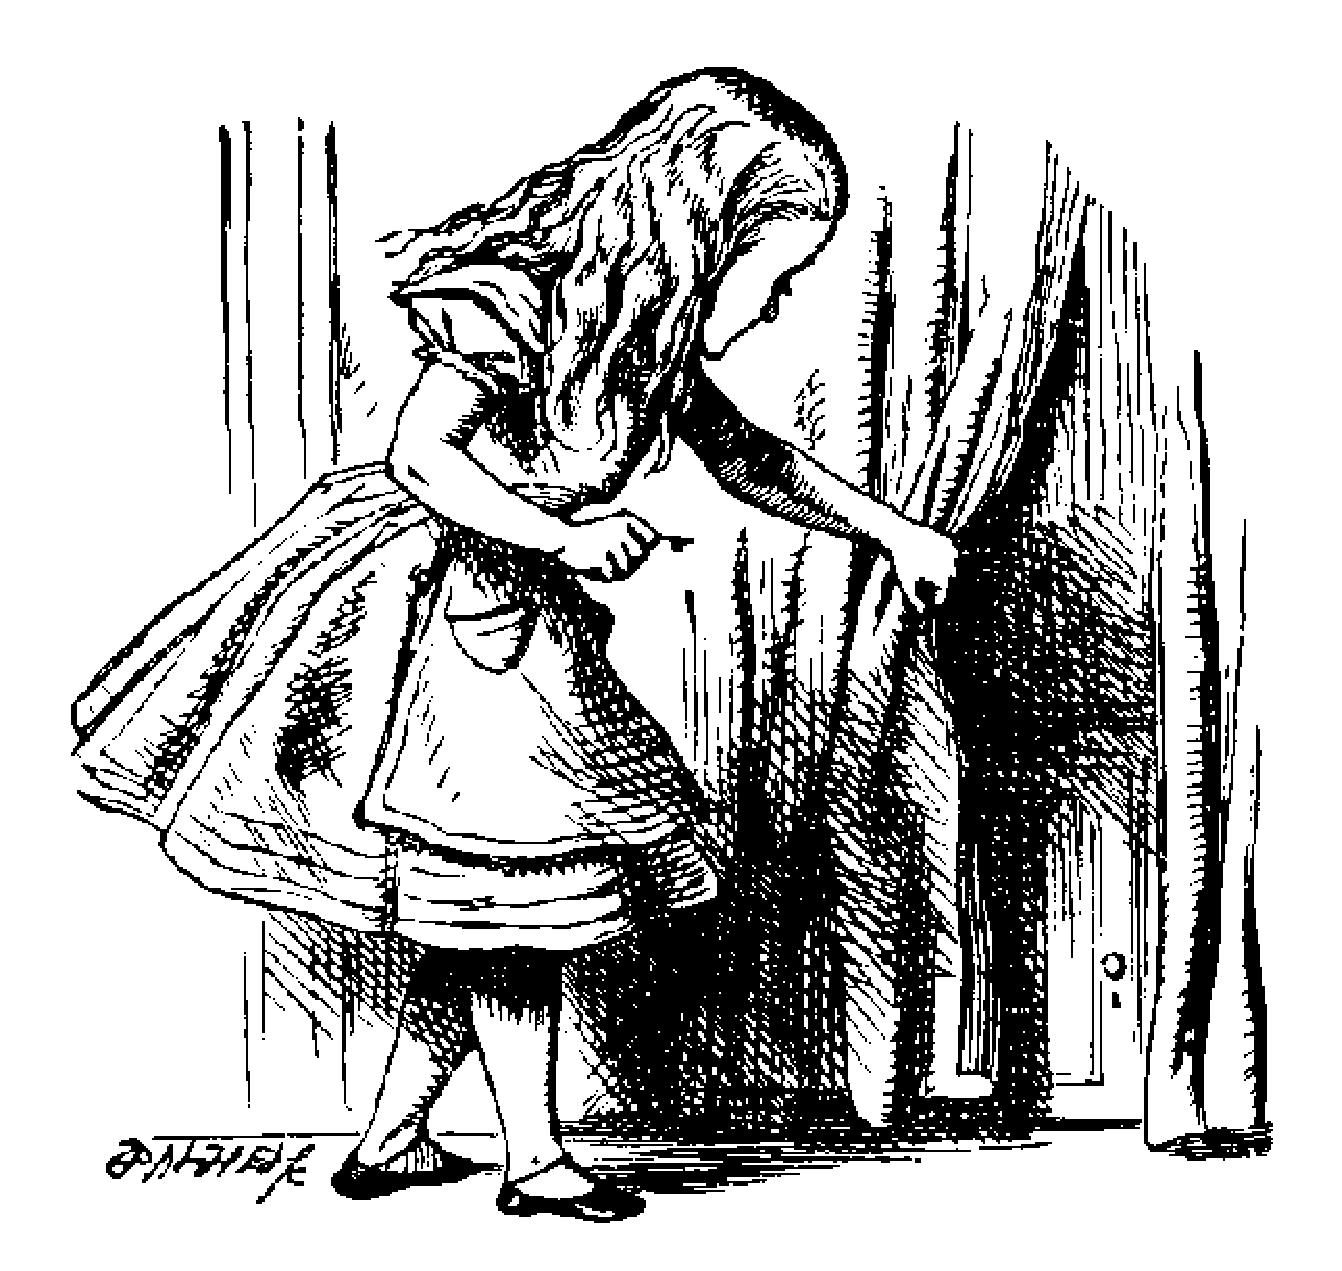
\includegraphics[scale=0.3]{alice.pdf}
\end{center}
\caption{\label{fig-eg}An example figure stretching over two columns}
\end{figure*}

\section{The WizWoz System}

Again, Simon Peyton Jones has a lovely description of how to write a
paper on his
website\footnote{\url{http://research.microsoft.com/en-us/um/people/simonpj/papers/giving-a-talk/giving-a-talk.htm}}.
Personally, I put URLs in footnotes and \emph{bona fide} references
in the bibliography. For instance, Turing \cite{turing37computable}
and Knuth \cite{knuth68art} would not be out of place in list of
references.
How many references? Hard to say. Five is not enough, 50 is pushing
it.


\section{Adversarial Graph Burning}
% define AGB formally (not sure if defining regular graph burning is needed formally?)

\subsection{Defining Adversarial Graph Burning}

First, we formalise the process of Adversarial Graph Burning on a graph $G$. Throughout, we presume that $G$ is a finite, simple, undirected graph.

\begin{definition}
\label{def/AGB}

Adversarial Graph Burning (or AGB for short) is a discrete-time graph process for two players. Each vertex is assigned one of 4 colours:

\begin{enumerate}
  \item \emph{White} vertices have not been burned by either player yet.
  \item \emph{Red} vertices have been burned by player 1.
  \item \emph{Blue} vertices have been burned by player 2.
  \item \emph{Green} vertices have been burned by \emph{both} players.
\end{enumerate}

At time $t=0$, all vertices are initially white. Each round consists of two main steps. First, both players simultaneously choose a white vertex, burning the vertex into that player's respective colour. Secondly, all non-white vertices spread their colour onto adjacent white vertices, according to the following rules:

\begin{itemize}
  \item If a white vertex is burned by multiple vertices, all with the same colour, the white vertex is also burned with the same colour.
  \item If a white vertex is burned by both red and blue vertices, the white vertex will become green.
  \item If a white vertex is burned by either red or blue vertices (but not both), and also by green vertices, the white vertex will become red or blue, respectively. 
\end{itemize}

\end{definition}

In particular, these rules ensure that this process is symmetrical, so the choice of player is unimportant.

Our main interest in this problem will be to count the maximum number of monochromatic components that can appear in any colouring of $G$ resulting from an instance of the AGB process. Our definition of "monochromatic components" differs slightly from most other uses of the term, so we define it separately here to account for these differences, and use slightly different terminology to emphasise these differences:

\begin{definition}
  \label{def/clusters}

Given a graph $G$, with an assignment of colours resulting from the AGB process, a \emph{red cluster} is a connected component in the subgraph induced by all red and green vertices in $G$. 

We also introduce the restriction that, in the AGB process, both players may only choose to burn the same vertex if there are no other remaining white vertices to burn.
\end{definition}

We note that only red clusters are defined here - blue clusters could of course be defined similarly, though since the AGB process is symmetrical we need only define red clusters.

In addition, the latter restriction on AGB is relatively minor, and mainly aims to remove some degenerate cases when counting red clusters, without needing to explicitly define exceptions for later results.

\subsection{Burning Sequences}

We now introduce a compact notation for describing a particular instance of adversarial graph burning.

\begin{definition}
\label{def/burning-sequence}

Given a graph $G$, a \emph{burning sequence} of length $n$, $B \in (V(G) \times V(G))^n$, is a sequence of tuples, $(r_1, b_1), (r_2, b_2), \dots, (r_n, b_n)$, such that player 1 burns vertex $r_t$ and player 2 burns vertex $b_t$ at time $t$.
\end{definition}

This sequence describes possible choices for the first $n$ rounds of the AGB process, but some further care is required to ensure this sequence describes valid choices for this process:

\begin{definition}
\label{def/valid-burning}

Given a burning sequence $B$, $B$ is said to be \emph{valid} if:

\begin{enumerate}
  \item For every vertex that appears in the $i^{th}$ term of $B$, say $v_i$, for every vertex in the $j^{th}$ term of $B$ such that $j < i$, say $v_j$ the distance between $v_i$ and $v_j$ is at most $(i-j)$.
  \item After the burning sequence described by $B$ is completed on $G$, every vertex is $G$ is non-white. 
\end{enumerate}

\end{definition}

From this definition, an immediate corollary is that the original graph burning problem is a subset of adversarial graph burning:

\begin{corollary}
\label{cor/burning-subset}

Given a valid burning sequence for the original graph burning problem, say $(v_1, v_2, \dots, v_n)$, the burning sequence $(v_1, v_1), (v_2, v_2), \dots, (v_n, v_n)$ describes a valid burning sequence in adversarial graph burning.

\end{corollary}

\subsection{Bounding the length of burning sequences}

A useful question in the adversarial graph burning problem is to consider the maximum number of rounds required for this process to terminate, providing an upper bound for the number of valid burning sequences for a graph $G$. The following result gives a useful bound for connected graphs:

\begin{theorem}
  \label{thm/connected-bound}
  For a connected graph $G$ with $n$ vertices, the maximum number of rounds required for the AGB process to terminate is $\lceil \frac{n}{3} \rceil$.
\end{theorem}

\begin{proof}
  Given a graph $G$, consider $U$, the subgraph induced by all white vertices in $G$. We aim to show that, if $U$ contains at least $3$ vertices, each round of AGB removes at least $3$ vertices from $U$.

  If $U$ contains at least $3$ vertices, then we choose $2$ vertices to initially burn, say $v_1$ and $v_2$, and we need to show that at least one other distinct vertex is adjacent to $v_1$ or $v_2$. Considering the possible degrees of $v_1$ and $v_2$ in $U$, there are two potentially problematic cases, while the other cases are straightforward.

  If $v_1$ and $v_2$ are both adjacent and have degree $1$, then no other vertices are adjacent to them. However, since $U$ has at least $3$ vertices, some other vertex $v_3$ must be in $U$, but not connected to $v_1$ or $v_2$. However, since $G$ is connected, $v_3$ must be adjacent to some non-white vertex in $G$, so $v_3$ must also be removed this round. A similar argument holds when $v_1$ and $v_2$ are both degree $0$.
  
  %If every vertex in $U$ is of degree at least $2$, then we are done - the two chosen vertices are removed from $U$, and at least one other vertex must be adjacent to these choices, and thus is removed.
  
  %If exactly one vertex in $U$ is of degree less than $2$, then by the restriction introduced in Definition \ref{def/clusters}, one of the chosen vertices has degree at least $2$, so at least $3$ vertices will be removed from $U$ this round.

  %If $U$ contains at least two vertices of degree $1$, if they are not adjacent we are done, since their adjacent vertices will also be removed. If they are adjacent, then either they are the only two vertices remaining, or there is another vertex that is not adjacent to either vertex of degree 1. Since $G$ is connected, this other vertex must be adjacent to a vertex that is not in $U$, so thise vertex will be removed on the same round as the two other chosen vertices.

  %If $U$ contains one vertex of degree $1$ and at least 1 vertex of degree $0$, then the vertex of degree $1$ must be adjacent to a vertex of degree at least $2$, so the above case holds. 

  %If $U$ only contains vertices of degree $0$, all of these vertices will be burned this round since they must be adjacent to previously burned vertices, so if there are at least $3$ vertices in $U$ then at least $3$ vertices will be removed from $U$ this round. 

  Hence, while at least $3$ vertices remain unburned, at least $3$ vertices are burned each round, and if there are ever less than $3$ vertices remaining they will all be burned in 1 round, so the maximum number of rounds to burn all vertices is $\lceil \frac{n}{3} \rceil$.
  
\end{proof}

\section{Counting Monochromatic Components}

\subsection{Monochromatic components on paths}

Our first key observation when counting red clusters is that at most one cluster can be added per round. This is because red vertices can be added in two different ways. If red vertices are added via spreading from adjacent vertices, no new clusters are created in this way (though existing clusters may be merged together, \emph{reducing} the number of red clusters on the graph). So red clusters can only be created by player 1 choosing vertices to burn, but only one vertex can be burned by player 1 each turn. Coupled with Theorem \ref{thm/connected-bound}, this gives a useful bound for the number of clusters on connected graphs:

\begin{corollary}
  \label{cor/path-clusters}

  Let $G$ be a connected graph on $n$ vertices. Then the maximum number of red clusters on $G$ is $\lceil \frac{n}{3} \rceil$, and this maximum is attainable when $G$ is a path on $n$ vertices.

\end{corollary}

\begin{proof}

Firstly, since each round can introduce at most 1 red cluster, and since the maximum number of rounds on $G$ is $\lceil \frac{n}{3} \rceil$ by Theorem \ref{thm/connected-bound}, the maximum number of red clusters on $G$ is $\lceil \frac{n}{3} \rceil$.

Now let $G$ be the path on $n$ vertices. Listing the vertices of $G$ in order from $v_1, v_2, \dots, v_n$, the burning sequence $(v_1, v_2), (v_4, v_5), \dots, (v_{n-2}, v_{n-1})$ contains $\lceil \frac{n}{3} \rceil$ red clusters.

%might add a diagram here?

\end{proof}

\subsection{Caterpillar graphs}

We now consider a natural extension of paths, and provide a method for counting clusters on these graphs.

\begin{definition}
  \label{def/caterpillars}

  A \emph{caterpillar graph} is a graph obtained by taking a path, and adding any number of vertices of degree 1 (known as leaves), that are adjacent to a vertex on the original path.

\end{definition}

In order to count clusters on caterpillar graphs, it will be useful to introduce more compact notation for describing caterpillar graphs:

\begin{definition}
  \label{def/caterpillar-strings}

  Given a caterpillar graph built on a path with $n$ vertices, its \emph{caterpillar string} is a sequence $C \in \mathbb{N}^n$ of the form $(c_1, \dots, c_n)$, where $c_i$ denotes the number of leaves adjacent to the $i^{th}$ path vertex. For instance, the caterpillar string $(1,0,2,3)$ represents the caterpillar graph shown in Figure [INSERT A PICTURE HERE].

\end{definition}

Clearly, there are a countably infinite number of caterpillar strings of length n. However, for the purposes of counting clusters, the following lemma shows that we can reduce the set of caterpillar strings to a finite subset of strings of a given form:

\begin{lemma}
  \label{lem/reduced-caterpillars}

  Given a caterpillar string $C$, the maximum number of red clusters in $C$ is equal to the maximum number of red clusters in the caterpillar string given by

  \begin{equation*}
  C'_i = \begin{cases}
    0 & C_i = 0 \\
    1 & C_i \geq 1
  \end{cases}
  \end{equation*}

  Moreover, given such a caterpillar string $C'$, if the first or last element in $C'$ is $1$, this can be removed and two zeros can be appended to the start or end of the sequence respectively, giving an equivalent caterpillar string, say $C''$. After performing these two operations, we say that $C''$ is a \emph{reduced caterpillar string}.
\end{lemma}

\begin{proof}

For the first reduction, suppose a given path vertex $v_i$ has at least $2$ adjacent leaves. Pick two of these leaves without loss of generality, calling them $l_1$ and $l_2$, and consider the subgraph induced by $v_i$, $l_1$ and $l_2$.

Suppose that this subgraph contains $2$ red clusters. Then both leaves must be coloured red. However, this is only possible when $v_i$ is also red. Since both leaf vertices are not adjacent, 2 rounds are required to colour them both red, and hence the first one coloured red will spread to $v_i$, colouring it red. And if $v_i$ was already coloured blue, it would spread its colour to at least one of $l_1$ and $l_2$, so by contradiction this subgraph can contain at most $1$ red cluster. And since the leaves were chosen without any loss of generality, either no leaves are red, all leaves are red along with their common path vertex, or exactly one leaf is red, so all but one leaf can be removed without changing the overall number of clusters.

For the second reduction, if one of the endpoints has a leaf, the leaf can be treated as a path vertex rather than a leaf vertex, removing a leaf from the existing endpoint and becoming the new endpoint instead.
% maybe a diagram here?
\end{proof}

Therefore, the set of reduced caterpillar strings of length $n$ is given by the set of bitstrings of length $n$ beginning and ending with a $0$, hence there are $2^{n-2}$ reduced caterpillar strings of length n. In practice this may be reduced even further, since reversing the reduced caterpillar string gives another string that may be different, but which always represents an isomorphic caterpillar graph.

\subsection{Monochromatic components on caterpillar graphs}

As discussed in Lemma \ref{lem/reduced-caterpillars}, we can transform any caterpillar graph into a reduced caterpillar graph while keeping the same number of maximum red clusters on the graph. We now present the following algorithm to count the maximum number of red clusters on any reduced caterpillar graph:

Given a reduced caterpillar string, partition this string into pieces of length 3, leaving any remainder characters in the last piece which may be shorter than 3 characters, and treat each of these pieces as a (not necessarily reduced) caterpillar string.

For each of these pieces, we can easily compute the maximum number of red clusters which originate in this piece, given some starting and ending constraints. These constraints are comprised of 4 distinct cases:

\begin{itemize}
  \item In case \emph{RW}, when colouring of this piece begins, the first path vertex is white, but the previous adjacent path vertex, which if it exists is not part of this piece, is coloured red.
  \item Case \emph{BW} is equivalent to case \emph{RW}, except the previous path vertex is blue instead of red. This is also the case applied for the very first piece, in order to ensure that colouring the first path vertex red correctly counts the start of a new red cluster.
  \item Case \emph{R} is where the first path vertex is already coloured red, since the colouring of the previous piece is not fully contained within that piece.
  \item Case \emph{B} is analogous to case \emph{R}.
\end{itemize}

These cases are defined for the start of a piece, but the ending constraints are analogous, and crucially correspond to the same starting constraint of the next piece.

Since these pieces are small, each of these computations is small and relatively simple to perform. For each piece, this then produces a weighted directed bipartite graph $G_P$, with vertex set $\{RW_{start}, BW_{start}, R_{start}, B_{start}, \\ RW_{end}, BW_{end}, R_{end}, B_{end}\}$, such that an edge exists from $X_{start}$ to $Y_{end}$ if there exists a colouring of piece $P$ with starting constraint $X$ and ending constraint $P$, with weight equal to the number of clusters originating in $P$.

Once all of these bipartite graphs are computed, the ending vertices of each piece can be merged with the starting vertices of the next piece, along with adding in a common source and sink vertex, removing every case bar case \emph{BW} from the first piece, generating a directed acyclic multipartite graph $G$. Then, the maximum number of red clusters on the reduced caterpillar graph is equal to the length of the longest path in $G$.

For future reference, we shall summarise this algorithm below:

\begin{definition}
\label{def/caterpillar-algorithm}
  Given a reduced caterpillar graph $G$, and assuming that each piece of length at most 3 has been pre-computed, a colouring for $G$ can be attained through the following algorithm:

  Partition the reduced caterpillar graph into as many connected subgraphs containing at most 3 path vertices as possible, leaving any remaining vertices in a piece at the end which may be shorter than length 3.

  For each piece, define a bipartite graph with vertices $$\{RW_{s}, BW_{s}, R_{s}, B_{s}, \\ RW_{e}, BW_{e}, R_{e}, B_{e}\}$$ such that an edge exists from $X_{s}$ to $Y_{e}$ with weight $w$ if the maximum number of red colourings originating this piece on a valid colouring with starting contraint $X$ and ending constraint $Y$ is $w$.

  After defining these graphs, define a multipartite graph $M$, merging the ending constraints of each piece and the corresponding starting constraint of the subsequent piece, along with adding source and sink vertices. Then the maximum number of red clusters on the reduced caterpillar graph is equal to the length of the longest path in $M$.
\end{definition}


Assuming that the bipartite graphs for each possible piece are pre-computed beforehand, producing the directed acyclic graph $G$ takes $O(p)$ time where $p$ is the number of pieces to combine, since each piece requires combining two constant sets of vertices together, along with constant time operations to add source and sink vertices. Since each piece adds at most $4$ additional vertices to $G$, and at most $16$ additional edges, the number of vertices and edges in $G$ are both $O(p)$. And finding the longest path in a directed acyclic graph with $V$ vertices and $E$ edges takes $O(V+E)$ time, this algorithm takes $O(p)$ time overall. But since each piece is of length at most 3, the number of pieces is linear in the length of the caterpillar, so this algorithm takes $O(n)$ time, being linear in the length of the reduced caterpillar string.


In order to justify the correctness of this method, namely that it provides the exact maximum number of red clusters attainable on $G$, we must first justifying colouring each piece in sequence.

\begin{lemma}
\label{lem/sequential-optimal}
For a (not necessarily reduced) caterpillar graph $G$ split into a series of pieces of length at most 3 as in the previous algorithm, say $P_1, \dots, P_n$, the optimal colouring in terms of maximising red clusters is attained by colouring $P_1$, then $P_2$, and so on up to $P_n$.
\end{lemma}
\begin{proof}
This proof proceeds by induction on the number of pieces in $G$.

 If $G$ has just one piece, then clearly colouring this piece will attain the optimal colouring, so the base case trivially holds.

 Now suppose the lemma holds for any (not necessarily reduced) caterpillar graph consisting of at most $n-1$ pieces. Then $G$, a caterpillar graph with $n$ pieces, is made up of the concatenation of two caterpillar graphs - one graph with $n-1$ pieces followed by one piece.

If either end piece is fully coloured first, the lemma holds from the inductive hypothesis. If a different piece is fully covered first, then $G$ is split into two smaller graphs, each with length less than $n-1$ pieces. If an optimal colouring for one of these graphs is attained using the inductive hypothesis, then the colouring will spread to the other piece, so it is not possible to colour each of these pieces sequentially - and hence, this colouring cannot be better than the optimal colouring, so the lemma holds in this case.

Now suppose the first piece coloured is not fully covered, so another piece starts being coloured before the first piece is finished. Then the possible colourings on this first piece are a subset of all possible colourings, so the number of red clusters on this first piece cannot be any better than optimal. Then applying the inductive hypothesis to the remaining pieces means that the result holds.

\end{proof}

Note that this lemma holds for caterpillar graphs even if they are not fully reduced - in particular, their strings need not start or end in a $0$. This allows induction to be applied, since concatenating non-reduced caterpillar graphs can still lead to a reduced caterpillar graph.

The algorithm being exact follows from this lemma, since the multipartite graph constructed during the algorithm describes all possible ways to colour the caterpillar graph sequentially, and since the longest path is chosen the most optimal way to colour the whole graph is chosen, even if this means deviating from the greedy approach.

\subsection{Graph diameter in adversarial graph burning}

A key heuristic when counting the maximal number of monochromatic components for a particular graph $G$ is the \emph{diameter} of $G$:

\begin{definition}
\label{def/diameter}
  Given a graph $G$ with vertex set $V(G)$, the \emph{diameter} of $G$ is given by
  
  \begin{align*}
  D(G) = \max_{u \in V(G), v \in V(G)} d(u,v)
  \end{align*}

  where $d(u,v)$ is the length of the shortest path between $u$ and $v$, and if no such path exists we say that $d(u,v) = \infty$.
\end{definition}

In the context of adversarial graph burning, this means that any instance of adversarial graph burning on $G$ will terminate within $D(G)$ rounds, when $G$ is connected. The following example suggests that graphs with low diameter tend to admit fewer clusters than high diameter graphs:

\begin{lemma}
\label{lem/cycle-clusters}
  Let $G$ be a cycle on $n$ vertices. Then the maximum number of red clusters on $G$ is $\lceil \frac{n}{4} \rceil$, and this bound is tight.
\end{lemma}

\begin{proof}
  Firstly, labelling the vertices of $G$ as $v_1, \dots, v_n$ in order, keeping in mind that $v_1$ is adjacent to $v_n$, the burning sequence $(v_1, v_n), (v_{n-2}, v_3), (v_5, v_{n-4}), \dots$ attains $\lceil \frac{n}{4} \rceil$ red clusters, since at each round except possibly the last, $4$ vertices are burned and $1$ new red cluster is started.

  Secondly, since every vertex has degree $2$, at least $4$ vertices must be burned every round, with the proof of this following a very similar structure to Corollary \ref{cor/path-clusters}. And since at most $1$ cluster can be created per round, the maximum number of red clusters on $G$ is at most $\lceil \frac{n}{4} \rceil$.
\end{proof}

In conjunction with Corollary \ref{cor/path-clusters}, the previous lemma presents a surprising fact: Since the maximum number of clusters on a path is $\lceil \frac{n}{3} \rceil$, and $\lceil \frac{n}{4}\rceil$ on a cycle, adding a single edge can reduce the maximum possible number of clusters on a graph by an arbitrary amount. This suggests that the diameter of a graph is important.

\subsection*{Counting monochromatic components in trees}

Compared to our previous work on paths and caterpillar trees, trees present some unique challenges when counting monochromatic components. In particular, our strategies for colouring paths and caterpillar trees generally rely on being able to limit the spread of vertices, and proceed through the graph in a clear sequence. However, in general trees do not possess a convenient start or end point, so such a sequence is not so clear to find. As a result, rather than the exact results in previous sections, we focus on approximate results for trees, improving on our existing upper bounds. Our first result uses that all trees contain caterpillar graphs:

\begin{definition}
  \label{def/maximal-caterpillar}
  Given a tree $T$, the \emph{maximal caterpillar of $T$}, denoted $C_T$, is the subgraph induced by all vertices in the longest path in $T$, along with all vertices which are distance $1$ from said path. If there are multiple longest paths in $T$, the maximal caterpillar of $T$ is induced by the path such that the number of vertices in the caterpillar is maximised.
\end{definition}

Once this caterpillar has been obtained, this can be coloured to attain a bound on red clusters for $T$:

\begin{corollary}
  \label{def/tree-caterpillar}
  Given a tree $T$, the maximum number of red clusters on $T$ is at least as many as the maximum number of red clusters on $C_T$.
\end{corollary}

\begin{proof}
  Consider the colouring on $C_T$ generated by our previous procedure - we claim this colouring can also be applied when $C_T$ is a subgraph of $T$. Every vertex in $T \setminus C_T$ is adjacent to at most one vertex in $C_T$, since being adjacent to more than one vertex would result in a cycle. Therefore, these vertices are only coloured when their adjacent vertex in $C_T$ is already coloured, so the colouring of $C_T$ is unaffected by these vertices.
\end{proof}

A natural suggestion is that the tightness of this bound depends on how many vertices of $T$ are included in the maximal caterpillar, which is discussed further in the following lemma:

\begin{lemma}
  \label{lem/ratio-tends-to-zero}
  For any tree $T$, denote the \emph{caterpillar ratio of $T$} as the number of vertices in $M_T$ divided by the number of vertices in $T$. This ratio can be arbitrarily close to zero.
\end{lemma}

\begin{proof}
Let $B_h$ be the perfect binary tree with height $h$. Then the longest path on $B_h$ is obtained by travelling between a leaf node in the left subtree of the root and a leaf node in the right subtree of the root, and this path has length $2h+1$. This path has $2(h-1)$ internal nodes, and each internal node has 2 children, with one child being included in the longest path and the other child being included in the maximum caterpillar, so the number of vertices in $M_{B_h}$ is equal to $4h-1$.

However, the number of vertices in $B_h$ is $2^{h+1}-1$, so the caterpillar ratio of $B_h$ is $\frac{4h-1}{2^{h+1}-1}$, which tends to $0$ as $h$ tends to $\infty$.
\end{proof}

%idea: find the longest path in the tree, take all vertices that are distance 1 away to find a caterpillar, consider remaining vertices

This shows that, while colouring the maximal caterpillar gives a lower bound on the maximum number of red clusters in a tree $G$, an arbitrarily large proportion of the graph is not contained within the maximal caterpillar. Hence, colouring the remainder of $G \setminus C_T$ will be key to obtaining a tighter lower bound on the maximum number of red clusters in $G$.

We first remark that $G \setminus C_T$ must be disconnected, since otherwise $G$ would contain a cycle. In particular, $G \setminus C_T$ is comprised of a set of connected components that are all trees, so an effective approach for colouring trees could be applied recursively by generating successively smaller caterpillars. This suggests one idea for an initial approach:

\begin{enumerate}
  \item Find the maximal caterpillar in $G$, $C_T$, and colour it using our previous techniques.
  \item Consider the subgraph of $G$ induced by white vertices, say $F$, which is a forest.
  \item Colour the tree in $F$ with greatest diameter, and repeat until the entire graph is coloured.
\end{enumerate}

This approach must eventually terminate, since each tree in $F$ must have lower diameter than the maximal caterpillar that defined it, or else the longest path defining the maximal caterpillar would contain some vertices in $F$.


Moreover, each tree in $F$ is adjacent to exactly one burned vertex - if it were adjacent to two or more burned vertices, this would define a cycle. We now use this fact to define some additional characteristics of each tree in $F$:

\begin{definition}
\label{def/roots}

Given a tree $T$ in $F$, a subgraph of a graph $G$ the \emph{root} of a tree, denoted $r_T$, is the vertex which is adjacent to an already burned vertex in $G$. The root is \emph{red-adjacent} if this burned vertex is red, with an analogous definition for a \emph{blue-adjacent} root. In addition, the \emph{rooted diameter} of $T$ is given by:

\begin{equation*}
rd(T) = 1 + \max_{v \in V(T)} d(r_{T},v)
\end{equation*} 

\end{definition}

From these definitions, it is apparent that, without choosing any vertices in $T$ to burn, any tree $T$ will be fully burned in $rd(T)$ rounds. As a corollary to this, the maximum number of clusters originating in $T$ is at most $rd(T)$. This provides an initial upper bound on the maximum number of red clusters in the graph $G$:

\begin{corollary}
\label{cor/root-distance-bound-1}
Consider a partial colouring of $G$ as produced by the above procedure, and the forest of unburned vertices $F$ comprised of a set of trees $\mathcal{T}$. Then the maximum number of red clusters on $F$ is at most $$\max_{T \in \mathcal{T}} rd(T)$$
\end{corollary}

Since this bound only considers the maximum rooted distance of any true, this can allow for significant simplification when considering many trees in a forest, particularly for small rooted distances. For instance, if every tree has rooted distance $1$, then every tree will be fully burned after 1 round. Therefore at most 1 cluster can be created, so as long as at least one tree has a blue-adjacent root.

{\bf Acknowledgments.}
Firstly, I would like to thank my supervisors - Jessica Enright, William Pettersson and John Sylvester - for their continual guidance and support throughout the project. I would also like to thank my parents, for always caring for me, and supporting my goals when I thought they could never be attained. And, last but not least, I would like to thank my girlfriend Jodie, for her never-ending love and kindness.

\bibliographystyle{abbrv}
\bibliography{example}


\end{document}